\documentclass[12pt, a4paper, onecolumn, twoside,french,cleardoublepage=plain,openany]{article}
\usepackage[french]{babel}
\usepackage[a4paper]{geometry}
\usepackage[utf8]{inputenc} % En unicode
\usepackage[T1]{fontenc}
\usepackage[pdfusetitle]{hyperref} % Pour les liens cliquables et metadata généré
\usepackage{indentfirst} % Linéa sur les premiers paragraphes
\usepackage[babel=true]{csquotes} % permet de faire \enquote{a} (« a »)
\usepackage{graphicx} % pour inclure les images
\usepackage[fleqn]{amsmath} % pour certains signes mathématiques
\usepackage{amssymb} % pour le signe de convolution
\usepackage[french,boxed,lined,onelanguage]{algorithm2e}
\SetAlCapSkip{1em} % Marge entre l'algo et le caption
%\SetAlCapNameSty{textit} % style du texte du caption des algos
\usepackage[toc,page]{appendix} % Annexes
\usepackage{fancyhdr} % Pour \lhead, \rhead... 
\usepackage[font={it}]{caption}
\usepackage{multirow} % Pour colonnes multiples des tableaux
\usepackage{pdfpages} % Include des pdfs
\usepackage[nottoc,numbib]{tocbibind} % Pour faire apparaitre la biblio. dans le sommaire
\usepackage[acronym,toc,shortcuts]{glossaries}
\usepackage[french]{cleveref} % permet de faire \cref au lieu de \ref
\usepackage{booktabs} % pour \toprule (un style de tableau)
\usepackage{float} % \begin{figure}[H] pour empêcher les figures de bouger

\usepackage[backend=bibtex,style=alphabetic,sorting=debug]{biblatex}
\bibliography{bibiographie.bib}
\newcommand{\code}{\texttt}

\begin{document}

\title{TER 45 \\ Aide humanitaire et logistique de crise : \\ Problèmes de couverture dans les graphes avec priorités}
\author{Abdelwahab Heba, Dimitry Berardi, Boris Terooatea, Maël Valais}
%\date{\today}
\maketitle
\tableofcontents

\section{Introduction}\label{introduction}
De tout temps, les catastrophes, qu’elles soient d’ordre naturelle, militaire ou sanitaire, ont touchées des population entières dans des régions aléatoires et de manière imprévisible. 

La logistique humanitaire intervient afin de mettre en place toute l’organisation matérielle en vue du bon déroulement d’une mission humanitaire, et se distingue de la logistique classique par les contraintes humaines qu'elle impose. 

Il convient de distinguer trois phases dans cette logistique :

La première : la phase de préparation , consiste à conserver un stock permanent pour permettre une réponse rapide à l’urgence.
La seconde : la phase de réponse à l'urgence , orientée vers la mise à disposition de ressources provisionnelles aux populations dans les zones sinistrées.
Et pour finir, la phase de reconstruction , celle-ci intervient dans le long terme et tire notamment une grande part de son savoir-faire dans les valeurs du développement durable.
Notre travail se concentrera essentiellement sur la seconde phase, la phase de “Réponse à l’urgence”.

\section{État de l'art}
\subsection{L'approche par couverture : le CTP} \label{CTP}

L’article \cite{gendreau_covering_1997} est le premier à introduire le CTP. Il s’agit d’un ensemble de noeuds à couvrir et un ensemble atteignable … Il cherche à construire une route pour un véhicule, et tous les points qui ne sont pas sur cette route sont atteignables facilement (sont proches). Cette route est construite en utilisant un seul véhicule qui peut faire le parcours entier. Par exemple, dans cette situation, le CTP pourrait être utilisé pour localiser les endroits optimaux pour placer des boîtes de poste, ou construire une route pour les équipes de réapprovisionnement de biens dans des pays en développement, dans lesquels les services médicaux ne peut être délivrés qu’à un ensemble de villages, mais où tous les utilisateurs sont capables de visiter cette équipe.

L’article \cite{hodgson_covering_1998} implémente le CTP de Gendreau \& al., et pour la première fois dans un cas réel : l’acheminement de biens vers des centres de réapprovisionnement au \enquote{Suhum District}, Ghana. Dans ce cas, il y a deux saisons : la saison sèche et la saison des pluies. Durant la seconde saison, certains noeuds accessibles durant la saison sèche deviennent inaccessible par la route, il faut donc pouvoir établir un nouveau parcours pour livrer un maximum d’habitats. Cet article s’intéresse donc à ce problème, en changeant le rayon de livraison des points de livraison.

L’article \cite{naji-azimi_covering_2012} concerne la localisation de centres de distributions satellites pour fournir de l’aide humanitaire à des gens atteints par un désastre dans un zone. Comme les équipes ne peuvent pas visiter tous les habitants, certains doivent se déplacer dans des centres de distributions satellites pour obtenir des biens pour leur survie, en prenant en compte que ces centres ne sont pas trop loin de chez eux, donc accessibles à pied. Ces centres doivent être réapprovisionnés depuis un dépôt central, par un ensemble de véhicules homogènes ayant une certaine capacité. Cet article introduit l’idée de diviser la livraison, et propose une approche heuristique pour résoudre le problème.


\subsection{Minimisation des coûts et facteurs humains : le CCVRP} \label{CCVRP}

L’article \cite{campbell_routing_2008} traite de l’approvisionnement des ressources critiques aux personnes qui en ont le plus besoin dans le cas d’une catastrophe naturelle sous un autre angle. Le fait que les livraisons soient critiques implique qu’elles soient rapides et juste envers les personnes touchées par un désastre. Cet article montre que le principe classique de minimisation des coûts n’est pas adapté dans le cas d’un désastre, et présente pour la première fois une méthode avec deux fonctions objectives différentes : minimiser le temps d’arrivée maximal et minimiser le temps d’arrivée moyen. Cet article offre le premier pas vers le développement d’outils de livraisons d’aide humanitaire.

L’article \cite{ngueveu_effective_2010} met en place le CCVRP, qui répond à un problème de transport cherchant à réduire la somme des temps d’arrivée aux clients. Cela s’applique notamment dans le cas où la priorité est donnée à la satisfaction des besoins des clients, comme par exemple l’approvisionnement en biens vitaux après une catastrophe naturelle. Elle propose alors un parcours à l’aide d’un ensemble de véhicules homogènes ayant une certaine capacité. Dans le CCVRP, le bonheur de chaque client est donc pris en compte.



\section{Analyse et proposition}

Comme le suggère \cite{campbell_routing_2008}, la minimisation des coûts lors du choix d’un itinéraire ne permet pas d’assurer des temps d’arrivée convenables lorsqu’il s’agit de distribution d’aide humanitaire d’urgence ; le CCVRP est un bon exemple de modèle prenant en compte cette problématique.

Le CTP répond à la problématique de l’accès aux sites de livraison dans le cas humanitaire, mais sans prendre en compte les temps d’arrivée sur les sites de distributions (noeuds atteignables). En effet, le CTP se base sur le modèle classique du voyageur de commerce (TSP) pour le choix de l’itinéraire.

Nous proposons donc une version du CTP intégrant, au lieu d’un TSP classique, un CCVRP.

\begin{table}[h] \centering \begin{tabular}{@{}ll@{}} \toprule
\multicolumn{1}{c}{CTP} & \multicolumn{1}{c}{CCVRP} \\ \midrule
Permet de prendre en compte des situations où tous les endroits (noeuds) ne sont pas atteignables, ou lorsqu'on ne souhaite visiter qu'un sous-ensemble de noeuds & Nécessite que tous les noeuds soient atteignables \\
Basé sur une minimisation des coûts & Basé sur une minimisation des temps d'arrivée \\ \bottomrule
\end{tabular} \caption{Tableau comparatif CTP vs. CCVRP} \label{comparatif}
\end{table}

\begin{figure}[H] \centering
	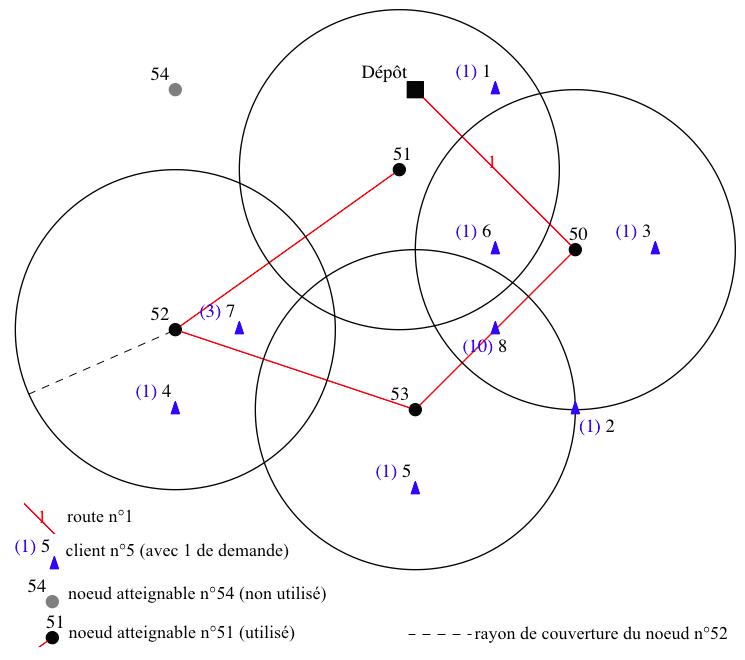
\includegraphics[width=0.999\textwidth]{figures/ctp_sans_vrp}
	\caption[]{Exemple de solution d'un CTP. Nous avons utilisé notre modèle de CTP-VRP en limitant le nombre de véhicules à un pour produire ce graphe.} \label{fig_ctp_sans_vrp} 
\end{figure}


\begin{figure}[H] \centering
	\centerline{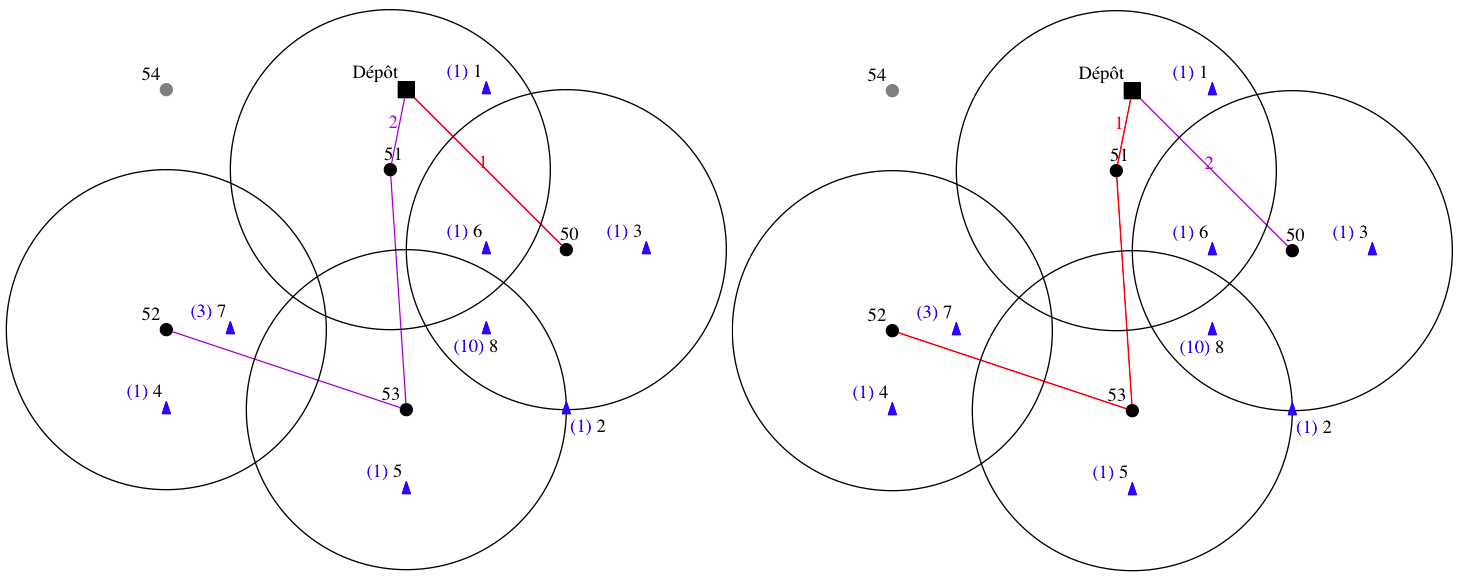
\includegraphics[width=1.3\textwidth]{figures/deux_camions_combines}}
	\caption[]{À gauche, la solution référence du CTP-VRP. À droite, la solution modèle proposé, le CTP-CCVRP} \label{fig_deux_camions}
\end{figure}

\begin{table}[H] \centering \begin{tabular}{@{}llll@{}} \toprule % utilise booktabs
 & CTP avec VRP & CTP avec CCVRP & Écart relatif \\ \midrule
Nombre de camions & 2 & 2 & +0,0\% \\
Distance parcourue & 17,09 & 17,09 & +0,0\% \\
Somme des temps d'arrivée & 15,07 & 15,07 & +0,0\% \\
Temps d'arrivée maximal & 7,19 & 7,19 & +0,0\% \\ \bottomrule
\end{tabular} \caption{Avec deux camions disponibles} \label{deux_camions}
\end{table}


\begin{figure}[H] \centering
	\centerline{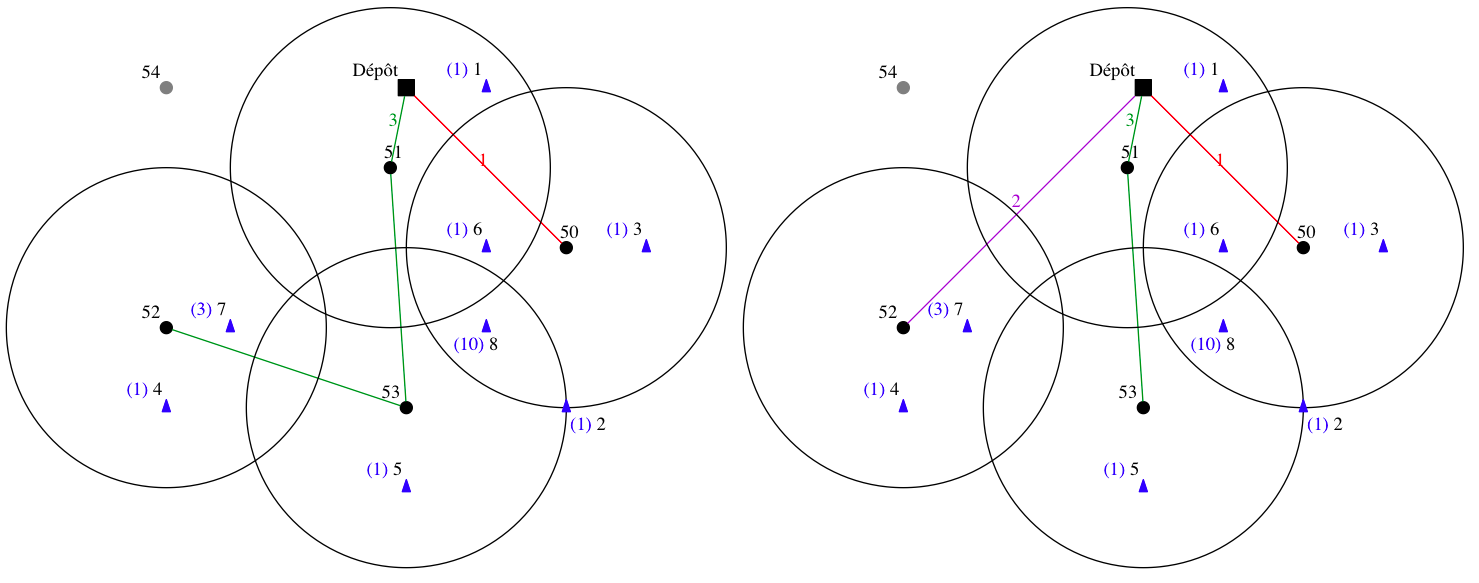
\includegraphics[width=1.3\textwidth]{figures/trois_camions_combines}}
	\caption[]{À gauche, la solution référence du CTP-VRP. À droite, la solution modèle proposé, le CTP-CCVRP} \label{fig_trois_camions}
\end{figure}


\begin{table}[H] \centering \begin{tabular}{@{}llll@{}} \toprule % utilise booktabs
 & CTP avec VRP & CTP avec CCVRP & Écart relatif \\ \midrule
Nombre de camions & 2 & 3 & +50,0\% \\
Distance parcourue & 17,09 & 22,17 & +29,7\% \\
Somme des temps d'arrivée & 15,07 & 12,12 & -19,6\% \\
Temps d'arrivée maximal & 7,19 & 4,24 & -41,0\% \\ \bottomrule
\end{tabular} \caption{Avec trois camions disponibles} \label{trois_camions}
\end{table}


\begin{figure}[H] \centering
	\centerline{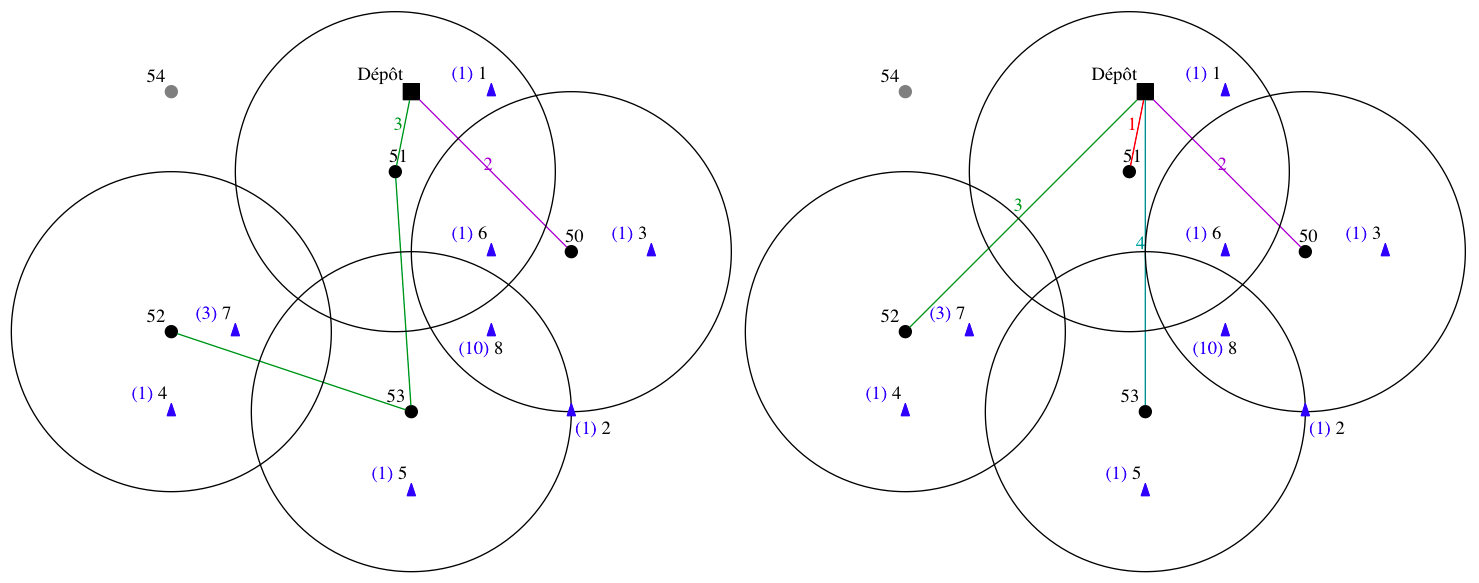
\includegraphics[width=1.3\textwidth]{figures/quatre_camions_combines}}
	\caption[]{À gauche, la solution référence du CTP-VRP. À droite, la solution modèle proposé, le CTP-CCVRP} \label{fig_trois_camions}
\end{figure}

\begin{table}[H] \centering \begin{tabular}{@{}llll@{}} \toprule % utilise booktabs
 & CTP avec VRP & CTP avec CCVRP & Écart relatif \\ \midrule
Nombre de camions & 2 & 4 & +100,0\% \\
Distance parcourue & 17,09 & 24,18 & +41,5\% \\
Somme des temps d'arrivée & 15,07 & 12,09 & -19,8\% \\
Temps d'arrivée maximal & 7,19 & 4,24 & -41,0\% \\ \bottomrule
\end{tabular} \caption{Avec quatre camions disponibles} \label{quatre_camions}
\end{table}

\section*{Annexes}
\subsection{Modèle mathématique du CTP-CCVRP}\label{modele}
\begin{equation}
Min \sum_{i=0}^{m}\sum_{j=0}^{m}\sum_{k=1}^{l}c_{ij}x_{ijk}
\end{equation}

s. t. :

\begin{equation}
\sum_{i=0}^{m}x_{ijk} = y_{jk}   j\in\left\{1,2,...,m\right\}, k\in\left\{1,2,...,l\right\}
\end{equation}

\begin{equation}
\sum_{i=0}^{m}x_{jik} = y_{jk}   j\in\left\{1,2,...,m\right\}, k\in\left\{1,2,...,l\right\}
\end{equation}

\begin{equation}
\sum_{j=0}^{m}x_{0jk} = 1   k\in\left\{1,2,...,l\right\}
\end{equation}

\begin{equation}
\sum_{j=0}^{m}x_{j0k} = 1   k\in\left\{1,2,...,l\right\}
\end{equation}

\begin{equation}
\sum_{j=1}^{m}\sum_{k=1}^{l}\alpha_{ij}D_{isjk} \geq d_{is}    i\in\left\{1,2,...,n\right\}, s\in\left\{1,2,...,t\right\}
\end{equation}

\begin{equation}
\sum_{i=1}^{n}\sum_{s=1}^{t}w{s}D_{isjk} \leq Q_{k}y_{jk}    k\in\left\{1,2,...,l\right\}, j\in\left\{1,2,...,m\right\}
\end{equation}

\begin{equation}
\sum_{s=1}^{t}\sum_{i=1}^{n}\sum_{j=1}^{m}w{s}D_{isjk} \leq Q_{k}    k\in\left\{1,2,...,l\right\}
\end{equation}

\begin{equation}
u_{ik} - u_{jk} + (m + 1)x_{ijk} \leq m   i,j\in\left\{1,2,...,m\right\}, k\in\left\{1,2,...,l\right\}
\end{equation}

\begin{equation}
x_{ijk} \in\left\{0,1\right\}   i,j\in\left\{1,2,...,m\right\}, k\in\left\{1,2,...,l\right\}
\end{equation}

\begin{equation}
y_{jk} \in\left\{0,1\right\}   j\in\left\{1,2,...,m\right\}, k\in\left\{1,2,...,l\right\}
\end{equation}

\begin{equation}
u_{ik} \geq 0   i\in\left\{1,2,...,m\right\}, k\in\left\{1,2,...,l\right\}
\end{equation}

\begin{equation}
D_{isjk} \geq 0   i\in\left\{1,2,...,n\right\}, s\in\left\{1,2,...,t\right\}, j\in\left\{1,2,...,m\right\}, k\in\left\{1,2,...,l\right\}
\end{equation}



\begin{equation}
u_{ik} - u_{jk} + Q_{k}x_{ijk} \leq Q_{k} - \sum_{s=1}^{t}\sum_{h=1}^{n}w_{s}D_{hsjk}   i,j\in\left\{1,2,...,m\right\}, k\in\left\{1,2,...,l\right\}
\end{equation}


\end{document}